\documentclass{article}
\usepackage[a4paper, total={6in, 8in}]{geometry}
\usepackage{graphicx}
\usepackage{hyperref}
\graphicspath{ {./temp/} }

\usepackage[utf8]{inputenc}

\title{CMSC 6950 Final Project - pymagicc}
\author{Behnam Farhadi}
\date{June 2021}

\begin{document}
\maketitle

\textbf{Abstract}

This report is provided for the final course course 6950. In this report, we have used the "Pymagicc" data to analyze two tasks. "Pymagicc" is a A Python wrapper for the simple climate model MAGICC. The first task is generate Radiative Forcing — Greenhouse Gases vs. year, and the second report is Generate Emissions—CO2—MAGICC AFOLU vs. Year. The result of each task is clearly specified in its output.

\vspace{1cm}
\section{Introduction}
Pymagicc is a Python interface for the Fortran-based reduced-complexity climate carbon cycle model MAGICC \cite{1}. Aiming at broadening the user base of MAGICC, Pymagicc provides a wrapper around the MAGICC binary, which runs on Windows and has been published under a Creative Commons Attribution. NonCommercial-ShareAlike 3.0 Unported License. Pymagicc itself is licensed under the GNU Affero General Public License v3.0 \cite{2}.
\vspace{1cm}
\section{Tasks}
In both tasks, we use the available data to examine the status of greenhouse gas emissions on a yearly basis. We sorted the available data and filtered the empty data from the tables. The results are clearly marked in the pictures. This project utilises the Pymagicc module to achieve the below computational tasks and visualizations.
\vspace{5cm} 
\subsection{ Task 1- Generate Radiative Forcing|Greenhouse Gases vs year}
In this task, Positive radiative forcing means Earth receives more incoming energy from sunlight than it radiates to space. This net gain of energy will cause warming.It can be concluded that despite all efforts, global warming is still a major threat. we read data from RCP26, RCP45, RCP60, RCP85 scenario files, convert the data in MAGICC data format to a pandas DataFrame, and then build visualizations to show Radiative Forcing|Greenhouse Gases for RCP26, RCP45, RCP60 and RCP 85 scenarios based on each year. 

\begin{figure}[h]
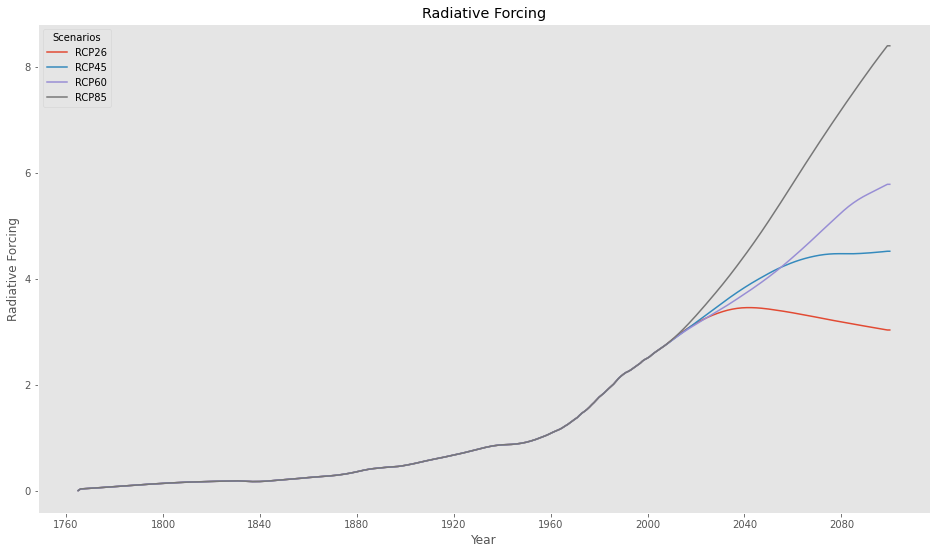
\includegraphics[width=\textwidth,height=\textheight,keepaspectratio]{Radioactive.png}
\end{figure}
 \begin{center}
\caption{Figure 1: Radiative Forcing by year based on RCP26, RCP45, RCP60 and RCP 85 data's}
\end{center}
\clearpage
\subsection{Task 2- Generate Emissions|CO2|MAGICC AFOLU vs Year}
Gases that trap heat in the atmosphere are called greenhouse gases. This section provides information on emissions of the main greenhouse gases like Co2.Also, AFOLU means "Agriculture, Forestry, and Other Land". The AFOLU sector is responsible for just under a quarter(~10-12 GtCO2eq/yr) of anthropogenic GHG emissions mainly from deforestation and agricultural emissions from livestock, soil and nutrient management (robust evidence; high agreement)\cite{4}
In this task, we run the MAGICC model on RCP26, RCP45, RCP60 and RCP85 scenarios and
visualize the Emissions|CO2|MAGICC AFOLU projections for each of the given projections from
1765 to 2100.
\begin{figure}[h]
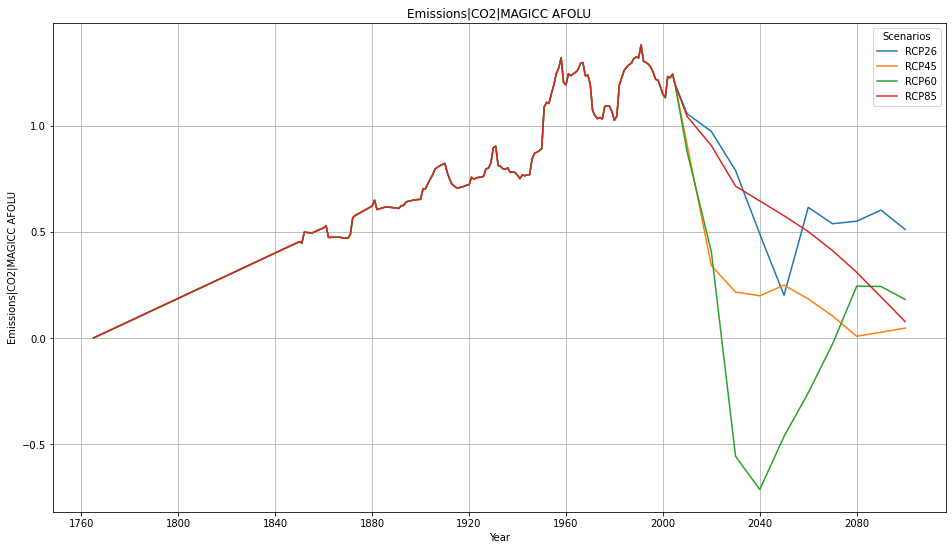
\includegraphics[width=\textwidth,height=\textheight,keepaspectratio]{Emmissions.png}
\end{figure}
 \begin{center}
\caption{Figure 2: enerate Emissions—CO2—MAGICC AFOLU by year based on RCP26, RCP45, RCP60 and RCP 85 data's}
\end{center}
\vspace{5cm} 
\section{How to Install}
First,we have to download the Miniforge3-Linux-x86\_64 from below link:\\

\href{https://github.com/conda-forge/miniforge/releases/latest/download/Miniforge3-Linux-x86_64.sh}https://github.com/conda-forge/miniforge/releases/latest/download/Miniforge3-Linux-x86\_64.sh\\

Then, we install it by this command: 
bash Miniforge3-Linux-x86\_64.sh  and then:\\

conda install matplotlib pandas seaborn notebook pymagicc\\

then:\\

sudo apt-get update \\

and:sudo dpkg --add-architecture i386\\

 last:\\
 sudo apt-get install wine
 Our environment for run pymagicc is ready know.\\
\vspace{1cm} 
\section{Conclusion}
In this report, we used the repository of "Pymagicc" software\cite{3}.You can get all the details about this program on the repository page. To implement, we used Google colab\cite{5}, which was an online platform for implementing and executing our commands. We also used pandas and matplotlib libraries. main data also called from "pymagicc".Two scenarios were implemented, one "enerate Radiative Forcing—Greenhouse Gases " and the other "enerate Emissions—CO2—MAGICC AFOLU". The results clearly show that the earth is still warming, although many efforts have been made to prevent it, but it is insufficient. This was a small part of the available data and parameters. Certainly more accurate results can be obtained by examining more parameters.

\vspace{0.5cm} 
\begin{thebibliography}{9}
\bibitem{1} 
Meinshausen, M., S. C. B. Raper, and T. M. L. Wigley. 2011. “Emulating Coupled
Atmosphere-Ocean and Carbon Cycle Models with a Simpler Model, MAGICC6 – Part 1:
Model Description and Calibration.” Atmospheric Chemistry and Physics 11 (4):1417–56.
https://doi.org/10.5194/acp-11-1417-2011
\bibitem{2} 
Gieseke et al., (2018). Pymagicc: A Python wrapper for the simple climate model MAGICC. Journal of Open Source Software, 3(22), 516.
https://doi.org/10.21105/joss.00516
\bibitem{3} 
https://github.com/openscm/pymagicc
\bibitem{4} 
https://www.ipcc.ch/site/assets/uploads/2018/02/ipcc_wg3_ar5_chapter11.pdf
\bibitem{5}
https://colab.research.google.com/
 
\end{thebibliography}
\end{document}

